\section{Bloc}\label{sec:bloc}
Bloc is an abbreviation of Business Logic Component and allows separating an application into separate layers.~\cite{bloc}
"The BLoC Pattern has been designed by Paolo Soares and Cong Hui, from Google and first presented during the DartConf 2018 (January 23--24, 2018)."~\cite{didierboelens}

"The goal of this package is to make it easy to implement the BLoC Design Pattern (Business Logic Component).

This design pattern helps to separate presentation from business logic.
Following the BLoC pattern facilitates testability and reusability.
This package abstracts reactive aspects of the pattern allowing developers to focus on converting events into states."~\cite{bloc}

Bloc is a library written by Felix Angelov and the concept bases on Reactive Programming.~\cite{bloc}
Bloc represents a control unit that is responsible for passing data from state into UI.
When a user clicks on a button, it throws an event action that Bloc detects and generates a new state.~\cite{bloc}
In a summary, a structure of the concept consists of the following parts in Bloc:
\begin{itemize}
    \item \textbf{Events} are the input to a Bloc.
    They are commonly UI events such as button presses.
    Events are added to the Bloc and then converted to States.
    \item \textbf{States} are the output of a Bloc.
    Presentation components can listen to the stream of states and redraw portions of themselves based on the given state (see BlocBuilder for more details).
    \item \textbf{Transitions} occur when an Event is added after mapEventToState has been called but before the Bloc's state has been updated.
    A Transition consists of the currentState, the event which was added, and the nextState.
    \item \textbf{BlocSupervisor} oversees Blocs and delegates to BlocDelegate.
    \item \textbf{BlocDelegate} handles events from all Blocs which are delegated by the BlocSupervisor.
    Can be used to intercept all Bloc events, transitions, and errors.
    It is a great way to handle logging/analytics as well as error handling universally.
\end{itemize}

\begin{figure}
    \centering
    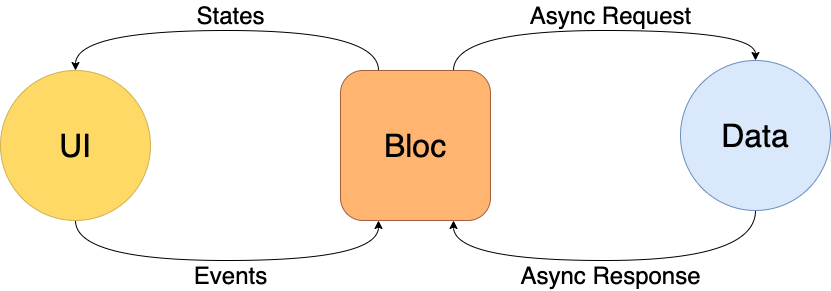
\includegraphics[scale=0.4]{assets/bloc_architecture.png}
    \caption{Bloc architecture~\cite{bloc}}
    \label{fig:bloc-architecture}
\end{figure}

\section{HydratedBloc}\label{sec:hydratedbloc}
"\textit{hydrated\_bloc}~\cite{hydratedBlocPubDev} is an extension to the \textit{bloc state management library}~\cite{bloc} which automatically persists and restores bloc states.

\textbf{hydrated\_bloc} exports a \textbf{HydratedStorage} interface which means it can work with any storage provider.
Out of the box, it comes with its own implementation: \textbf{HydratedBlocStorage}.

\textbf{HydratedBlocStorage} is built on top of \textit{path\_provider}~\cite{pathProvider} for a platform-agnostic storage layer.
The out-of-the-box storage implementation reads/writes to file using the \textbf{toJson/fromJson} methods on \textbf{HydratedBloc} and should perform very well for most use-cases (performance reports coming soon).
\textbf{HydratedBlocStorage} is supported for desktop (\textit{example}~\cite{hydratedBlocExample})."~\cite{hydratedBlocTut}

HydratedBloc works as well as common Bloc.
The difference is in data storage.
Hydrated Bloc allows us to store data through a JSON object.
So, whenever an application loads data, it is necessary to wait and show the user progress indicator, but it can show stored data immediately.
When it receives data, it will simply render it into a screen.

"\textbf{HydratedBlocStorage} is an implementation of \textit{HydratedStorage} which uses \textit{PathProvider} and \textit{dart.io} to persist and retrieve state changes from the local device."~\cite{hydratedBlocStorage}
So, it is a part of Hydrated Bloc implementation.